\documentclass[10pt,twocolumn,letterpaper]{article}

\usepackage{cvpr}
\usepackage{times}
\usepackage{epsfig}
\usepackage{graphicx}
\usepackage{amsmath}
\usepackage{amssymb}
\usepackage{caption}
\usepackage{subcaption}

% Include other packages here, before hyperref.

% If you comment hyperref and then uncomment it, you should delete
% egpaper.aux before re-running latex.  (Or just hit 'q' on the first latex
% run, let it finish, and you should be clear).
\usepackage[breaklinks=true,bookmarks=false]{hyperref}

\cvprfinalcopy % *** Uncomment this line for the final submission

\def\cvprPaperID{****} % *** Enter the CVPR Paper ID here
\def\httilde{\mbox{\tt\raisebox{-.5ex}{\symbol{126}}}}

% Pages are numbered in submission mode, and unnumbered in camera-ready
%\ifcvprfinal\pagestyle{empty}\fi
%\setcounter{page}{4321}
\begin{document}

%%%%%%%%% TITLE
\title{Cameras Simulating Lidar through CNN}

\author{Zhenghao Fei\\
BAE, UC, Davis\\
{\tt\small zfei@ucdavis.edu}
% For a paper whose authors are all at the same institution,
% omit the following lines up until the closing ``}''.
% Additional authors and addresses can be added with ``\and'',
% just like the second author.
% To save space, use either the email address or home page, not both
\and
Chen Peng\\
MAE, UC, Davis\\
{\tt\small penchen@ucdavis.edu}
\and
Shubo Chen\\
ECE, UC, Davis\\
{\tt\small sbochen@ucdavis.edu}
}
\maketitle
%\thispagestyle{empty}

%%%%%%%%% ABSTRACT
\begin{abstract}
Depth information are crucial in areas such as obstacle avoidance, autonomous mapping, route planning and navigation. Among various depth sensors that are currently available in the market, Lidars are popularly used in measuring depth information to surrounding environment because of its accuracy, precision and flexibility. However, Lidars can be very costly. In this project, we attempted to use convolutional neural network to train a two-eye camera with depth information detected from a 2D Lidar to see if the camera would learn how to extract depth information from images it captures so it could be a potential substitution of the expensive lidar. As in our knowledge, we are the first attempt that uses two images of a two-eye camera(generates two images at a time) as input to train a network to simulate lidar behavior so far. 
\end{abstract}

%%%%%%%%% BODY TEXT
\section{Introduction}

Depth information are crucial in areas such as obstacle avoidance, autonomous mapping, route planning and navigation. Among various depth sensors that are currently available in the market, Lidars are popularly used in measuring depth information to surrounding environment because of its accuracy, precision and flexibility. However, Lidars can be very costly. As from the papers we read\cite{kyto2011method},\cite{jones2011head}, \cite{diebel2004simultaneous} we learned that stereo cameras are able to detect depth information and they are relatively cheap compared to most of depth sensors, but previous methods like triangulation are not very effective in terms of accuracy and computational cost. Therefore, we propose this approach that trains a deep neural network on two cameras to obtain accurate depth values from targeted area just like what the precise sensors do. For this project, we run a ZED two-eye camera and an 2D lidar on a robotic system simultaneously in order to obtain images and lidar measured points. Then we use measured depth as ground truth, images as inputs to train a deep neutral network so that the images can be transformed to lidar points. We used ROS(Robotic Operating System) to monitor and control the camera and lidar and all the data were manually collected and stored by the team. 34K data were used as training data which was fed into the network and 1.5K data were used to perform validation. The network was constructed and operated in Tensorflow. The idea from this project may be extended to use some latent information obtained from sensor A to learn obvious and useful information from sensor B. Images contain much of such latent features of objects which can be extracted by DNN, just like human eyes do.
%-------------------------------------------------------------------------
\section{Related work}
Our work mainly focus on how to design neural network to extract useful visual representations of depth information from two pictures and calculate the regression value of  2-D depth in front of the robots.
\subsection{Traditional methods to calculate depth from two images}
In paper \cite{saxena2007depth}, they use images from two cameras to triangulate and estimate distances relative to robot and they also use monocular visual cues in the pictures to do the estimation. The conclusion suggests that the depth information indeed hide in two stereo camera pictures. Therefore, we can theoretically estimate the depth information from a stereo camera pair.  

\subsection{Supervised learning}

In paper \cite{pinto2016curious}, the author design a Siamese neural network to predict pushing angle and force exerting point on a object by inputting two pictures: object before pushing, object after pushing. Here they use 4 layers CNN and two connected fully connected network to predict 6 output regression values. In addition, they also use one row CNN to calculate the  predicted regression value of material hardness features of objects (slope and intercept of supporting force line). In this paper, the author mainly use the updated weights to do image recognition, but not testify the accuracy of their regression prediction. In paper [data-driven], they use NYU Depth v2 [indoor] dataset to train the DNN to extract an accurate dense 3D interpretation based on one single picture. They show the good result of dense information extracted from pictures, but the labels of dataset is also from Microsoft Kinect stereo camera, which are also calculated from classic methods and not as accurate as 2-D lidar. In our method, we use more accurate depth labels obtained by Lidar directly and expect to achieve better results. 
\section{Approach}
To construct our own datasets, we install a Zed camera and 2D Lidar on a small robot vehicle. The robots can be controlled to move in a complex depth changing environment. While robot’s moving, we record the input data: images captured by Zed camera and training labels: 2-D Lidar depth information.
\subsection{Robot platform}
To construct our own datasets, we install a Zed camera and 2D Lidar on a small robot vehicle. The robots can be controlled to move in a complex depth changing environment. While robot’s moving, we record the input data: images captured by Zed camera and training labels: 2-D Lidar depth information.
\subsubsection{Cameras}
We use Zed camera to capture environmental information in front of it, which can capture almost 10 pictures in one second. \textbf{Here we only use Zed camera to collect pictures in front of it.} As we talked in last chapter, the depth information lies in the two images they captured. The picture size taken by camera is 376*672*3 and the lidar we use is 2D, so we assume that the useful depth information at the height of 2D lidar sensing lies in the vertical middle one-third area of whole images taken by cameras. Therefore, we sliced the images to 128*672*3 as raw image inputs. The Zed camera is shown in Figure\ref{zed_camera}
\begin{figure}[t]
	\begin{center}
		%\fbox{\rule{0pt}{2in} \rule{0.9\linewidth}{0pt}}
		\includegraphics[width=0.8\linewidth]{pictures/zedcamera.png}
	\end{center}
	\caption{Zed Cameras}
	\label{zed_camera}
\end{figure}


\subsubsection{Lidar}
We use RPLIDAR, a 2D lidar to sense the depth information at its sensing height. 2-D Lidar can sense the depth information 360 degree of its around environment.The lidar is shown in Figure \ref{lidar}he sensing result is visualized in Figure\ref{lidar_sensing}.

\begin{figure}
	\centering
		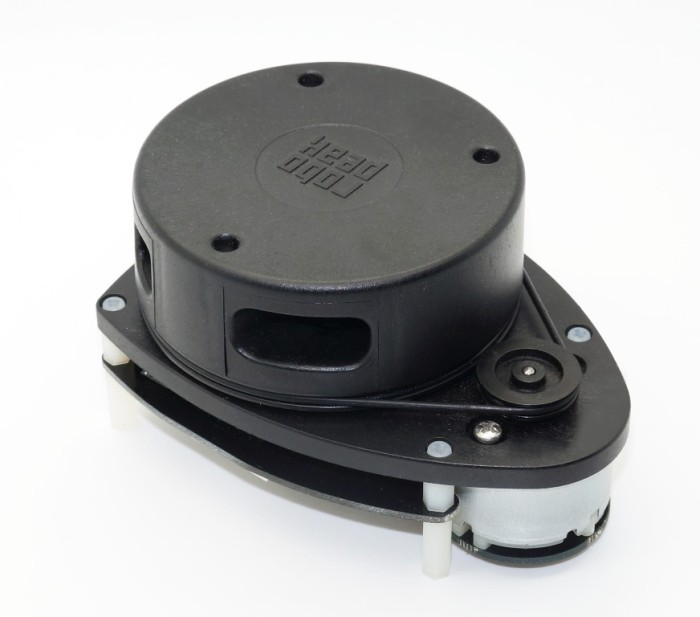
\includegraphics[width=.3\linewidth]{pictures/lidar.jpg}
		\caption{RPLIDAR 2D lidar}
		\label{lidar}

\end{figure}
\begin{figure}
		\centering
		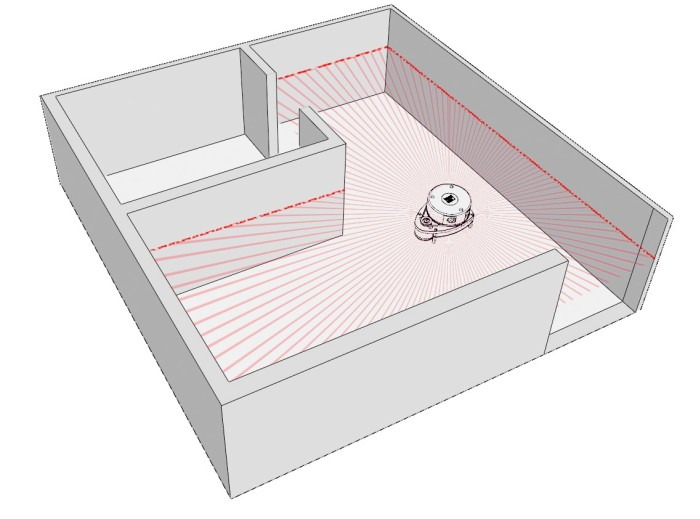
\includegraphics[width=.8\linewidth]{pictures/lidar_sensing.jpg}
		\caption{Another figure}
		\label{lidar_sensing}
\end{figure}

As the span view of the zed camera is 120 degree, therefore we choose the 120 degree depth information in front of cameras as labels. The lidar can obtain almost 5 pieces of depth information in 360 degree. 
%Mermin's description of how to write mathematics:
%\url{http://www.pamitc.org/documents/mermin.pdf}.
\subsubsection{ROS}
In order to collect the pictures taken by Zed camera and depth information recorded by Lidar, we use Robot Operating System (ROS) system to pack all the pictures and depth information in the series of recording time. ROS is a flexible framework for writing robot software. It is a collection of tools, libraries, and conventions that aim to simplify the task of creating complex and robust robot behavior across a wide variety of robotic platforms\cite{ROSabout}. We construct a ros node for lidar to publish the depth information and construct a ros node for zed camera to publish two compressed images taken by the two cameras. At the same time, we constructed a subscriber to record all the information and pack them into ros bags. After data collection, we use ‘rosbag play’ to publish all the captured images and depth information in time series. Meanwhile, we subscribe the publishing and keep the record of all data. At last, we matches all the images and depth labels based on recording time.  In figure \ref{two_images}, they show the two sliced images captured by camera, while in figure \ref{lidar_visual}, it shows the lidar depth information. The red area means the depth data we choose as labels.
\begin{figure}[t]
\begin{center}
%\fbox{\rule{0pt}{2in} \rule{0.9\linewidth}{0pt}}
\includegraphics[width=0.8\linewidth]{pictures/two_images.png}
\end{center}
   \caption{Two images taken by Zed camera at an instant}
\label{two_images}
\end{figure}

\begin{figure}[t]
	\begin{center}
		\includegraphics[width=0.8\linewidth]{pictures/lidar_visual.png}
	\end{center}
	\caption{Lidar Depth information}
	\label{lidar_visual}
\end{figure}

\section{Network Architecture}
Here we describe our network architecture for extract depth information from two images. The network architecture is showed in Figure X below. We tuned the size of images and convolutional filters during our experiments but keep the main structure same as this.

\begin{figure}
\centering
   \caption{Our convolutional neural network architecture for lidar simulating}
   \includegraphics[width=8cm]{pictures/network_architecture.png}
\label{network}
\end{figure}

\textbf{Two stream input:} Our task needs information from both left and right images so the network has two input streams to deal with two images. Unlike siamese network, the upper stream and lower stream don’t share weights. In this way the convolutional neural network is allowed to process two image differently which make more sense since two images has different viewpoints. 


\textbf{Extract edges, features, objects and scene:} The convolutional layers are used for edge and feature extraction, these information may help the network to better predict the depth. If we use a deeper convolutional network architecture the higher level notion of object and scene can also be used by the network. We think that with the help of edge, feature, object and scene notion, we can better extract depth information from images than the traditional way.


textbf{Regression:} The fully connected layers are used for nonlinear regression, we hope it can figure out the tradition way of triangulate and estimate distances. Different from many applications of using convolutional neural work to do classification, our network is doing regression job. It seems harder than classification, but we keep it in order to get more accurate gradient information from RMSE loss function rather than use a cross-entropy loss.


At this stage, we choose a relatively simple architecture to verify our idea, since a simple architecture is easier to train and need less amount of data to overcome overfitting. We can increase the depth when we have more data and want to achieve a better accuracy. 


Training details:Our convolutional neural network is implemented in Tensorflow  with a GTX 960 GPU. The training data has 34K examples and the validation set Is 1.5K. We use Gradient Descent Optimizer with learning rate decay factor 0.1 every 10000 epochs. 

\section{Results}


\section{Conclusion}
In this project we trained a neural network to learn how to extract depth information from images in order to determine if a cheap stereo camera can simulate the functionality of an 2D Lidar. With the experiments and results, we demonstrated that as more training data was fed in the network, the loss was decreasing, showing that the network is learning depth information from the given inputs and labels. However, from the figure of rmse of validation dataset, it is obvious that after the best score (1.79m), the model started overfitting. Possible explanations are that our training dataset is not large enough or the network is too complex. 

\section{Future Work}

In future work, we will first look at the issue of overfitting. Possible solutions are enlarge our training dataset and borrow other pre-trained CNNs and fine tune their architecture to fit our goal. Meanwhile, we will find a way to visualize the weights and outputs to see what we have learned to help us have a better understanding of the process. 

{\small
\bibliographystyle{ieee}
\bibliography{egbib}
}

\end{document}
